% 插入第8章PEO3–PPO4–PEO3组成段后；本片段不自动修改第8章。
% 全部引用Online原生截图，以独立LaTeX矩形裁切排版，不修改像素。
\begin{figure}[H]
\centering
% 100%浏览器图的核心参数(980,580,2040,1030)，1060×450；105mm约256ppi。
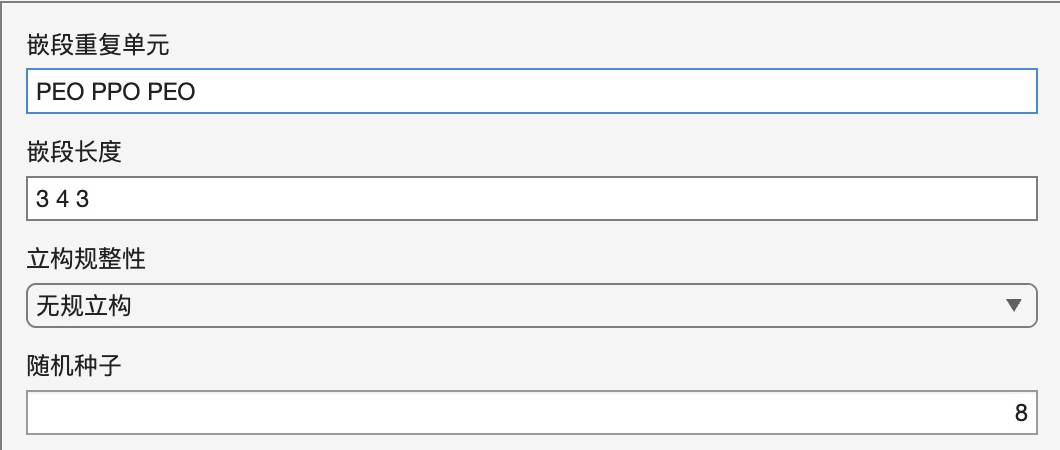
\includegraphics[width=105mm]{publication-assets/crop-3d7aab6f859860340b2f.png}
\par\vspace{3mm}
% 125%浏览器图中下部完整字段(845,710,2175,1535)，1330×825；122mm约277ppi。
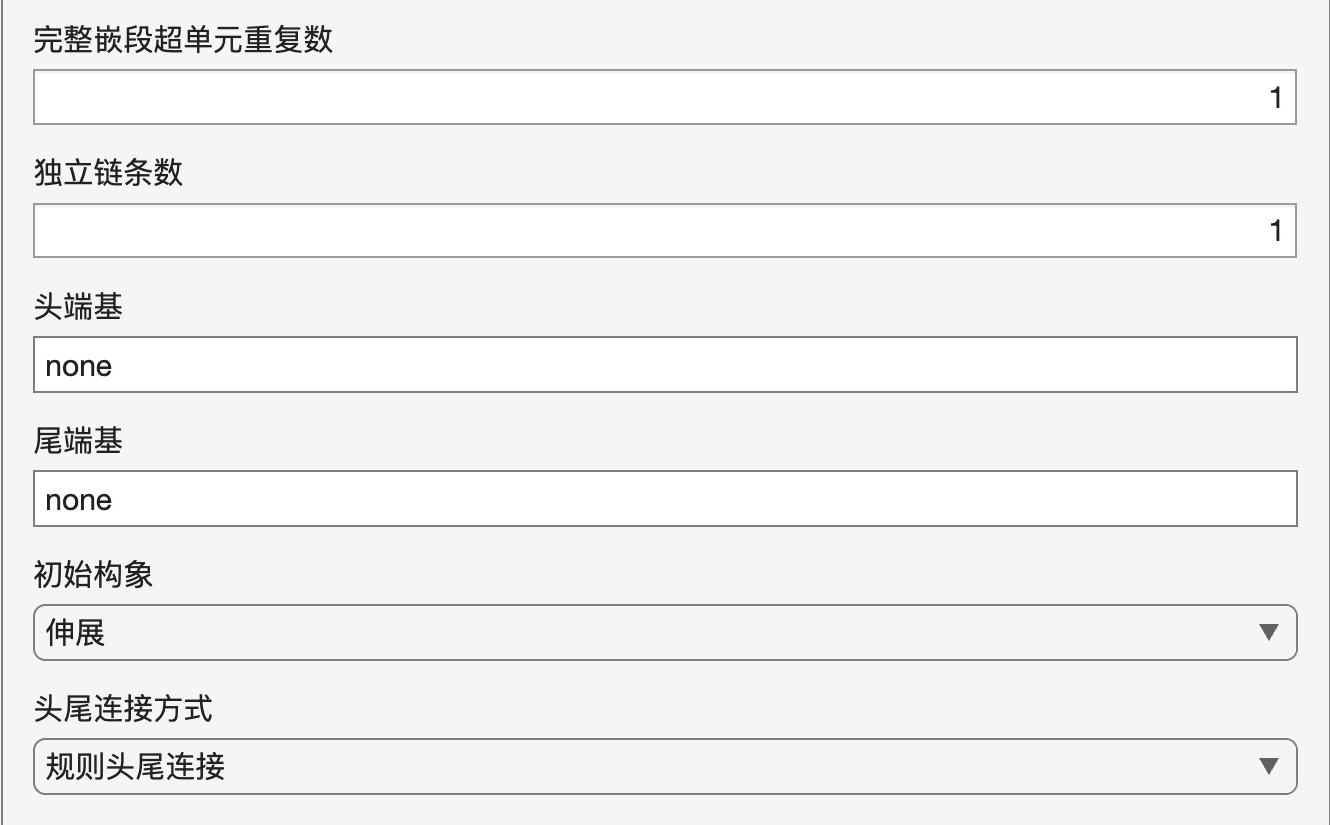
\includegraphics[width=\linewidth]{publication-assets/crop-14436d05d0623e7cdc6f.png}
\caption{Online中构建PEO--PPO--PEO嵌段链的实际参数局部。上方输入\literalinput{PEO PPO PEO}、\literalinput{3 4 3}和种子8；下方设为重复1次、1条链、首尾端基均为\file{none}，初始构象为伸展，采用规则头尾连接。两幅来自同一设置窗口在不同浏览器缩放下的实际画面。}
\label{fig:polymer-block-parameters}
\end{figure}

\begin{figure}[H]
\centering
% 完整链(165,900,2860,1150)，2695×250；122mm约561ppi。
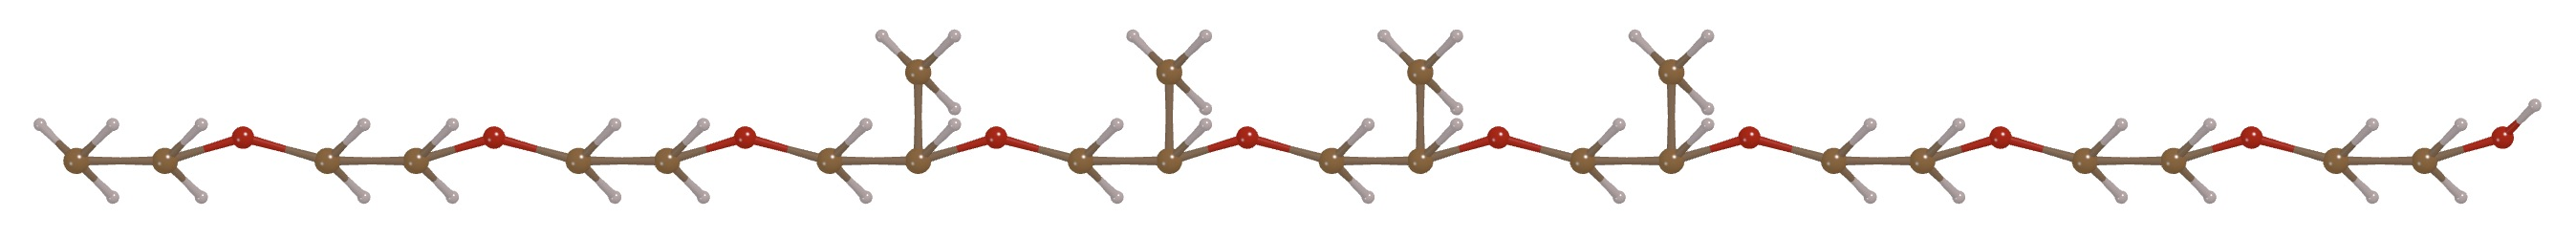
\includegraphics[width=\linewidth]{publication-assets/crop-7684a8a790954b6a1954.png}
\par\vspace{3mm}
\begin{minipage}[t]{40mm}
\vspace{0pt}
% 实际组成摘要(40,330,440,560)，400×230；40mm约254ppi。
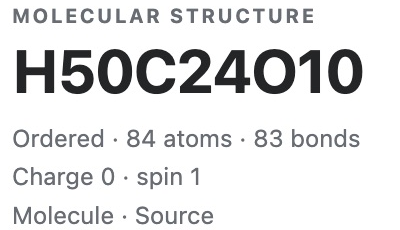
\includegraphics[width=\linewidth]{publication-assets/crop-c77f26280735587ce6a4.png}
\end{minipage}\hfill
\begin{minipage}[t]{80mm}
\vspace{0pt}
% 中部带四个甲基侧支的PPO局部(1000,900,2080,1150)，1080×250；80mm约343ppi。
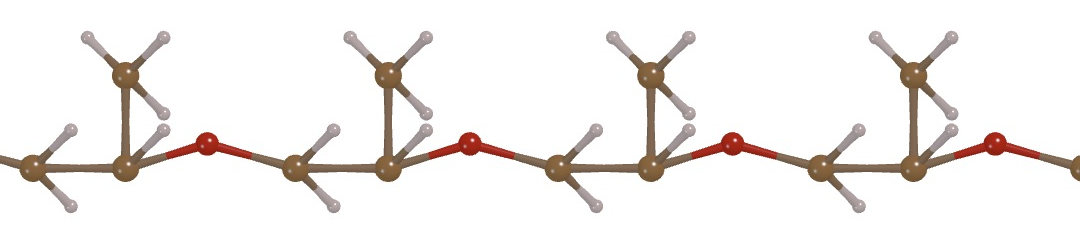
\includegraphics[width=\linewidth]{publication-assets/crop-71a6b6056b817444ef97.png}
\end{minipage}
\caption{应用上述参数后得到的实际嵌段链。上方显示整条链；下方左侧摘要为$\mathrm{C_{24}H_{50}O_{10}}$、84个原子和83条连接，右侧放大中部PPO段的四个甲基侧支。该图用于核对初始链的组成与连接，尚未进行几何优化或电子结构计算。}
\label{fig:polymer-block-model}
\end{figure}
